\documentclass[12pt]{article}

\usepackage[utf8]{inputenc}
\usepackage[T1]{fontenc}
\usepackage[slovak]{babel}
\usepackage{graphicx}

\title{Dokumentácia Hry \textit{Art of Magic}}
\author{}
\date{}

\begin{document}

\maketitle

\section{Úvod}
\textit{Art of Magic}  je jedinečná strategická kartová hra, kde sú hráči posudzovaní po každej bitke, pričom sa hodnotí ich výkon v dueli. Hodnotenie je založené na rôznych aspektoch ich hry, vrátane zostávajúceho zdravia po bitke, počtu použitých kariet určitej triedy a ďalších kľúčových momentoch stratégie a taktiky. Sudcovia analyzujú tieto faktory, aby vydali verdikt, ktorý môže ovplyvniť budúce hry a stratégie účastníkov.

\section{Základné Pravidlá}
\subsection*{Začiatok Hry}
Hráči začínajú s predom pripravenými balíčkami po 30 kartách. Cieľom hry je používať svoje karty na zníženie zdravia protivníka na nulu.

\subsection{Priebeh Hry}
Hráči striedavo ťahajú karty z balíčka a minú manu na hranie kariet. Karty môžu byť použité na útok proti protivníkovi alebo obranu, zmenu pravidiel hry alebo ovplyvnenie herného poľa.

\subsection{Vynesení Verdiktu}
Po ukončení duelu sudcovia (môžu byť AI alebo iní hráči, ktorí sa na dueli nezúčastňujú) analyzujú hru a vynášajú verdikt, ktorý môže ovplyvniť konečný výsledok. Verdikt môže zohľadňovať rôzne aspekty hry, ako je použitie kariet, strategické rozhodnutia a dokonca štýl hry.

\section{Režimy Hry}
\subsection{3.1 Jednohráčová Hra}
Hráč proti počítaču, kde počítač vystupuje v úlohe protivníka. Sudcovia môžu byť AI alebo diváci-hráči v online režime.

\subsection{Viachráčový Režim}
Hráči súperia proti sebe v online režime. Sudcovia, vybraní z radov divákov alebo automaticky určení, sledujú priebeh hry a po jej skončení vynášajú verdikt.

\section{Balíčky a Karty}
\subsection*{Vytvorenie Balíčka}
Hráči môžu vytvárať svoje balíčky, vyberajúc z širokej ponuky kariet. Vyvážený balíček zahŕňa bytosti, kúzla a artefakty, každý s unikátnymi schopnosťami.

\subsection{Typy Kariet}
\begin{itemize}
    \item Bytosti: Používajú sa na útok proti protivníkovi a obranu.
    \item Kúzla: Poskytujú rôzne efekty, od poškodenia po liečenie.
    \item Artefakty: Ponúkajú jedinečné výhody alebo menia pravidlá hry.
\end{itemize}

\section{Rozhranie Hry}
Herné rozhranie \textit{Art of Magic} je navrhnuté tak, aby bolo intuitívne a ľahko použiteľné, umožňujúce hráčom ľahký prístup k svojim kartám a prehľad o stave duelu.

\section{Záver}
\textit{Art of Magic} ponúka hlboký a pútavý herný zážitok, kde strategické myslenie a taktické rozhodovanie sú kľúčom k víťazstvu. Pripravte svoj balíček a dokážte svoje majstrovstvo v magických dueli v "Art of Magic".

\newpage
\section{Diagram tried}
\begin{figure}[h]
\centering 
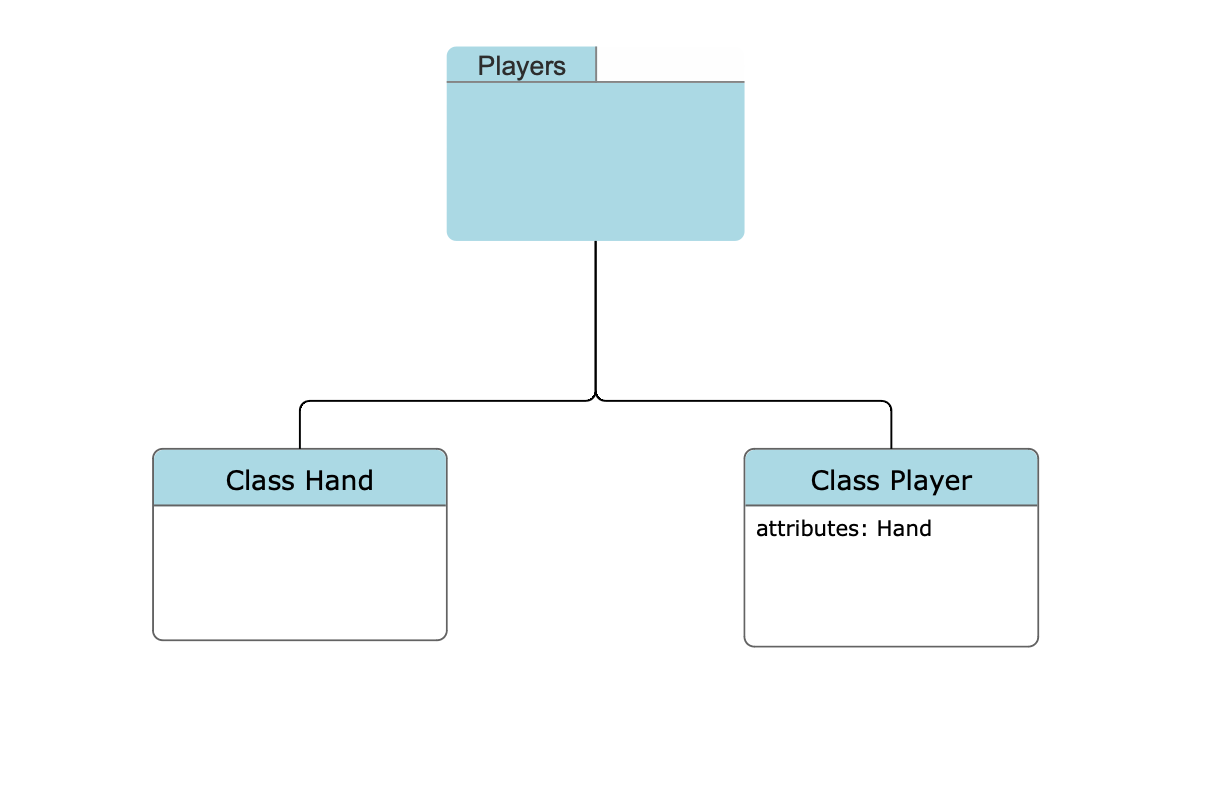
\includegraphics[width=0.5\textwidth]{img/1.png}
\end{figure}
\begin{figure}[h]
\centering 
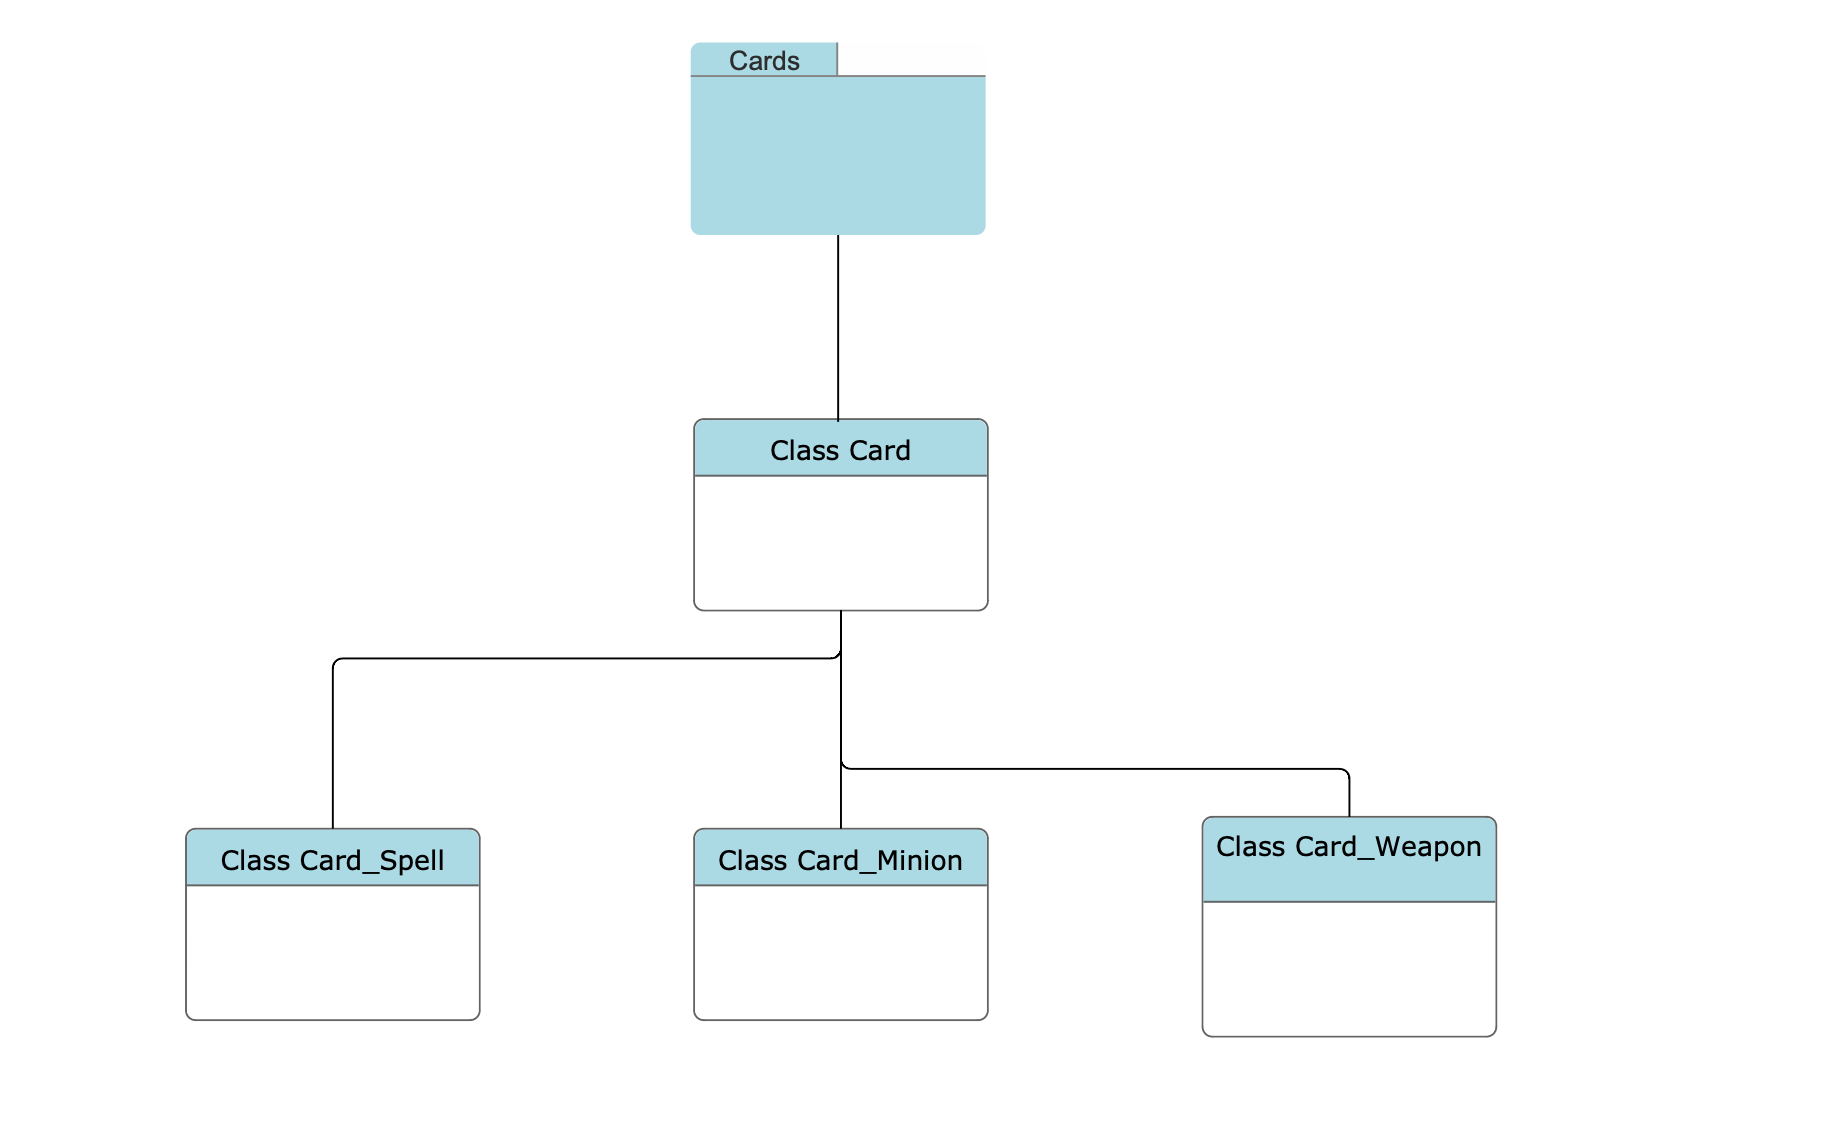
\includegraphics[width=0.5\textwidth]{img/2.png}
\end{figure}
\begin{figure}[h]
\centering 
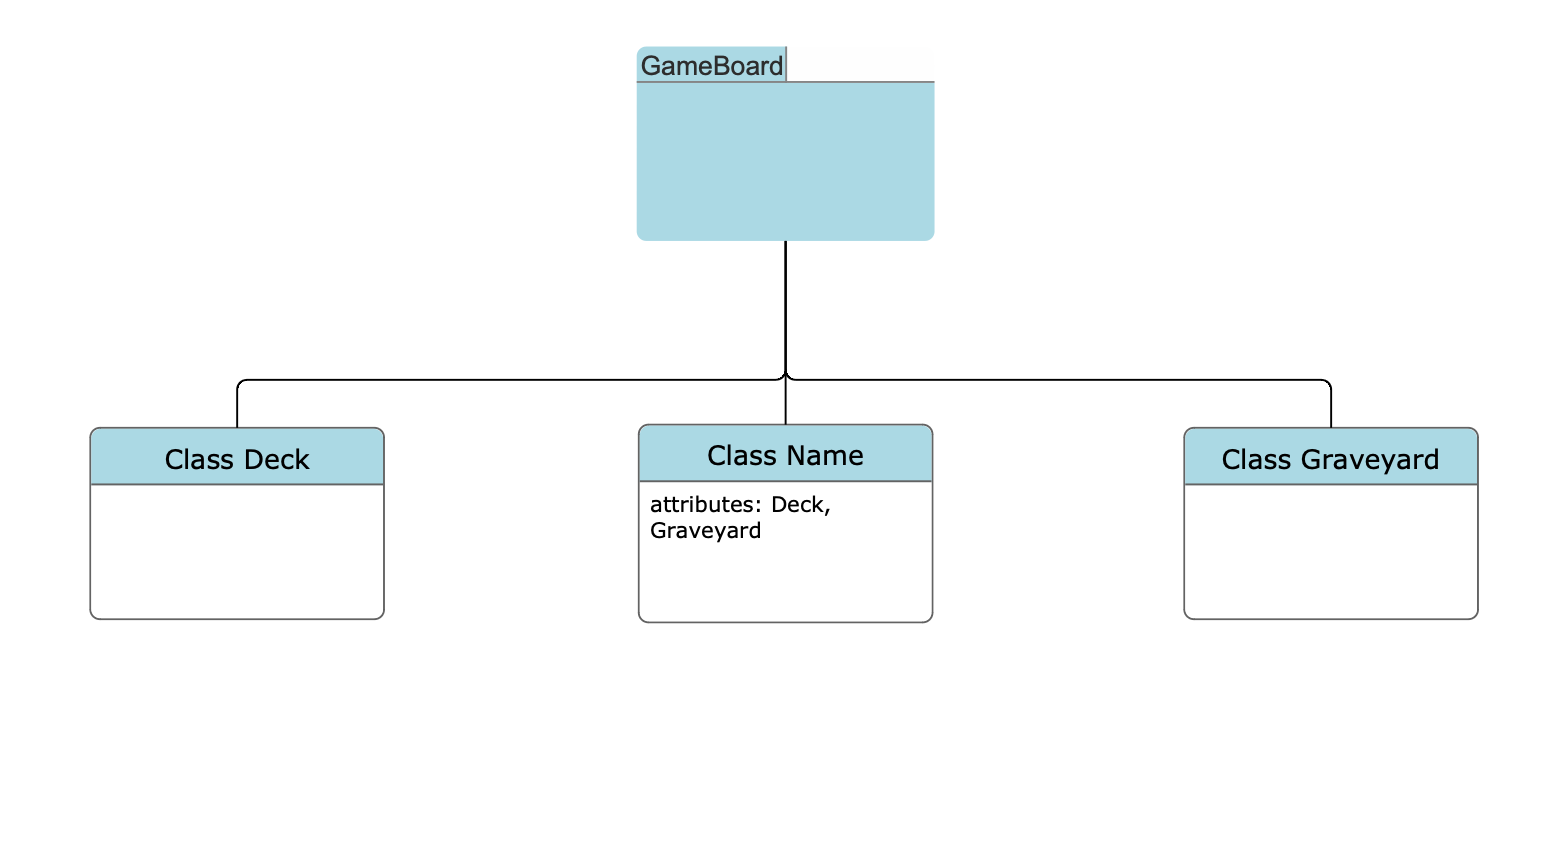
\includegraphics[width=0.5\textwidth]{img/3.png}
\end{figure}

\end{document}
